\documentclass[11pt]{beamer}


\usepackage[latin1]{inputenc}
\usepackage[french]{babel}
\usepackage[T1]{fontenc}

\usepackage{listings}
\usetheme{Warsaw}


\usepackage{tikz}
\usepackage{tikz-3dplot}
\usetikzlibrary{arrows,automata,shapes,snakes,graphs,positioning,calc}
\usepackage{tikz-qtree}

\tikzstyle{vertex}=[draw,fill=black!15,circle,minimum size=20pt,inner sep=0pt]

\tikzset{
        treenode/.style = {align=center, inner sep=0pt, text centered,font=\sffamily},
        arn_n/.style = {treenode, circle, white,font=\sffamily\bfseries, draw=black,
                fill=black, text width=1.5em},% arbre rouge noir, noeud noir
        arn_r/.style = {treenode, circle, red, draw=red,
                text width=1.5em, very thick},% arbre rouge noir, noeud rouge
        arn_x/.style = {treenode, rectangle, draw=black,
                minimum width=0.5em, minimum height=0.5em},%arbre rouge noir, nil
        arn_b/.style = {treenode, circle, black, draw=black, text width=1.5em},% arbre rouge noir, noeud noir
        arn_p/.style = {treenode, circle, white,font=\sffamily\bfseries, draw=black,
                fill=black, text width=1.5em},% arbre rouge noir, noeud noir
        cross/.style={cross out, draw=black, minimum size=2*(#1-\pgflinewidth), inner sep=0pt, outer sep=0pt},
        %default radius will be 1pt. 
        cross/.default={1pt},
        transition/.style={thick,->},
        arc_r/.style={bend angle=15,bend right,above left},
        arc_l/.style={bend angle=15,bend left,above right}
}



\title[Journey from userspace to kernel-land]{Linux debugging and tracing tools}
\author{Jugurtha BELKALEM}
\institute{SMILE - Opensource solution}
\date{\today}

\addtobeamertemplate{navigation symbols}{}{%
    \usebeamerfont{footline}%
    \usebeamercolor[fg]{footline}%
    \hspace{1em}%
    \insertframenumber/\inserttotalframenumber
}


\newcommand\Fontvi{\fontsize{6}{7.2}\selectfont}






\definecolor{mGreen}{rgb}{0,0.6,0}
\definecolor{mGray}{rgb}{0.5,0.5,0.5}
\definecolor{mPurple}{rgb}{0.58,0,0.82}
\definecolor{backgroundColour}{rgb}{0.95,0.95,0.92}


\lstdefinestyle{CStyle}{
    backgroundcolor=\color{backgroundColour},   
    commentstyle=\color{mGreen},
    keywordstyle=\color{magenta},
    numberstyle=\tiny\color{mGray},
    stringstyle=\color{mPurple},
    basicstyle=\footnotesize,
    breakatwhitespace=false,         
    breaklines=true,                 
    captionpos=b,                    
    keepspaces=true,                 
    numbers=left,                    
    numbersep=5pt,                  
    showspaces=false,                
    showstringspaces=false,
    showtabs=false,                  
    tabsize=2,
    language=C
}





\begin{document}
\logo{
\includegraphics[scale=0.20]{img/smile.png}}

\begin{frame}[plain]
\frametitle{Final Year Project Defense}
\framesubtitle{Master 2 Degree - Software for embedded systems}
\titlepage
\end{frame}


\AtBeginSection[]

{

  \begin{frame}[plain]

  \frametitle{Agenda}

  \tableofcontents[currentsection, hideothersubsections]

  \end{frame} 

}


\section{Introduction}
    \begin{frame}
\frametitle{Final Year Project Defense}

\framesubtitle{Master 2 Degree - Software for embedded systems}



 
 
 
 
 
\begin{columns}[t]

\hspace{15px}
\begin{column}{3cm}

\begin{alertblock}{Quotes}

UNIX is very simple, it just needs a genius to understand its simplicity.



\end{alertblock}

\end{column}

\hspace{60px}
\begin{column}{10cm}
\hspace{10px} {\Large How difficult is Linux?}
\vspace{15px}
	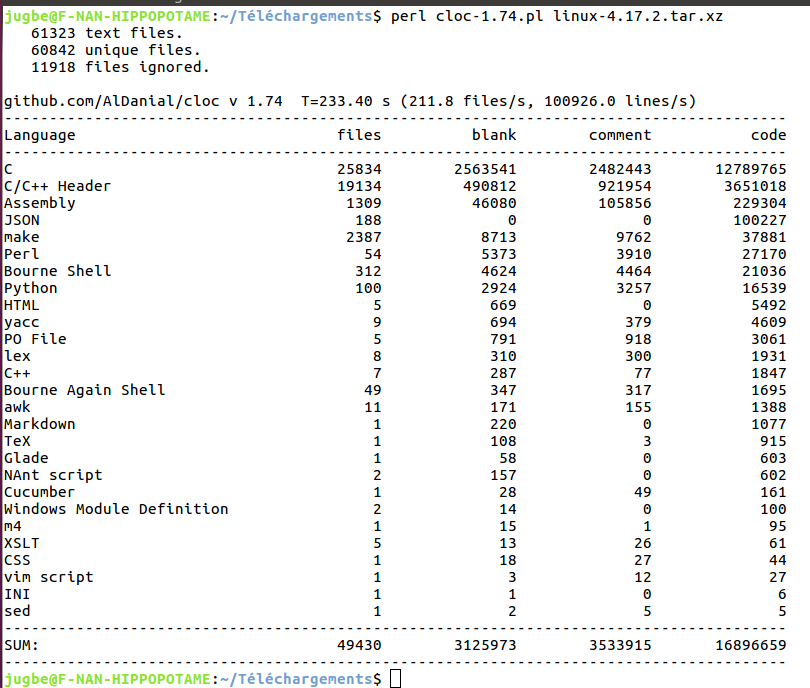
\includegraphics[scale=0.20]{img/linux-number-lines-of-code.png}

\end{column}


\end{columns} 
 

    \end{frame}



\section{Userland debugging mechanisms}

    \begin{frame}
\frametitle{Final Year Project Defense}

\framesubtitle{Master 2 Degree - Software for embedded systems}
    
    
    
    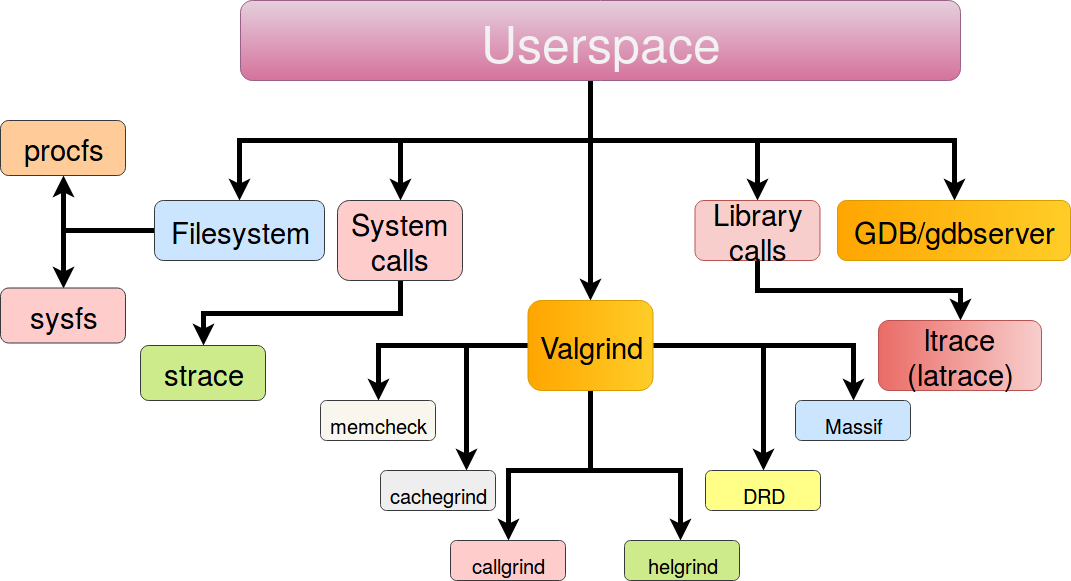
\includegraphics[scale=0.20]{img/userspace.png}
    
    

    \end{frame}


\section{Kernel code debugging}

    \begin{frame}
\frametitle{Final Year Project Defense}

\framesubtitle{Master 2 Degree - Software for embedded systems}
 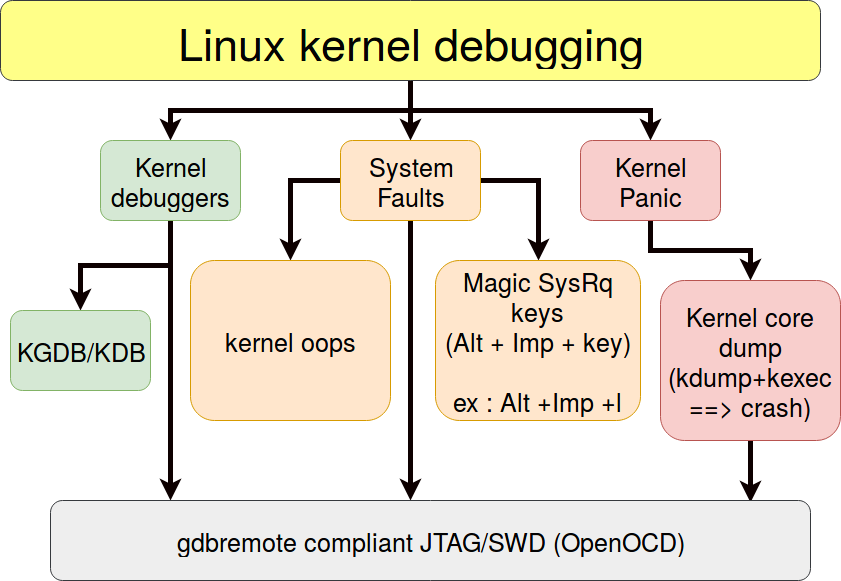
\includegraphics[scale=0.20]{img/kernel-debugging-ways1.png}

    \end{frame}


\section{Linux tracers}

    \begin{frame}
\frametitle{Final Year Project Defense}

\framesubtitle{Master 2 Degree - Software for embedded systems}
    %Linux tracers
\begin{figure}
        \resizebox{200pt}{!}{%
                \begin{tikzpicture}
                        %Plan z=0
                        \draw (0,0,0)   node[state]   (000) {$FTrace$};
                        \uncover<2->{\draw (5,0,0)   node[state]   (100) {$1,0,0$};}
                        \uncover<3->{\draw (10,0,0)  node[state]   (200) {$2,0,0$};}
                        \uncover<4->{\draw (15,0,0)  node[state]   (300) {$3,0,0$};}
                        \uncover<10->{\draw (0,5,0)   node[state]   (010) {$0,1,0$};}
                        \uncover<10->{\draw (5,5,0)   node[state]   (110) {$1,1,0$};}
                        \uncover<10->{\draw (10,5,0)  node[state]   (210) {$2,1,0$};}
                        \uncover<10->{\draw (15,5,0)  node[state]   (310) {$3,1,0$};}
                        \uncover<12->{\draw (0,10,0)   node[state]   (020) {$0,2,0$};}
                        \uncover<12->{\draw (5,10,0)   node[state]   (120) {$1,2,0$};}
                        \uncover<12->{\draw (10,10,0)  node[state]   (220) {$2,2,0$};}
                        \uncover<12->{\draw (15,10,0)  node[state]   (320) {$3,2,0$};}
         \end{tikzpicture}
        }
        \caption{Linux tracers}
        \end{figure}




    \end{frame}


\section{Reverse Anti-debug}

    \begin{frame}
\frametitle{Final Year Project Defense}

\framesubtitle{Master 2 Degree - Software for embedded systems}
 
 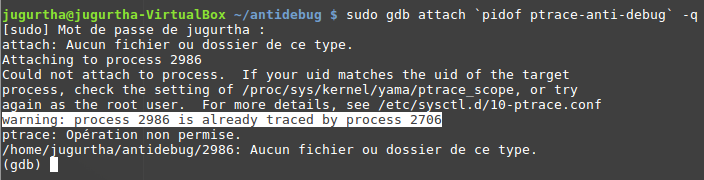
\includegraphics[scale=0.20]{img/gdb-cannot-be-attached.png}   
   
    \end{frame}


\section{Conclusion}

    \begin{frame}
\frametitle{Final Year Project Defense}

\framesubtitle{Master 2 Degree - Software for embedded systems}
    Conclusion

    \end{frame}

    
    
\section{Results from intership}

    \begin{frame}
\frametitle{Final Year Project Defense}

\framesubtitle{Master 2 Degree - Software for embedded systems}
    At the end of internship :
    \begin{itemize}
    	\item Step by step debugging manual (over 200 pages) + sample codes at : {\color{blue} \url{https://github.com/jugurthab/Linux_kernel_debug}}
    	 
    	 \item {4 articles on SMILE's blog : }
    	 \begin{itemize}
    	    \Fontvi
    	 	\item \textbf{OpenOCD from scratch : } {\color{blue}\url{http://www.linuxembedded.fr/2018/07/openocd-from-scratch/}}

    	 	\item \textbf{Linux debugging tools : } {\color{blue}\url{http://www.linuxembedded.fr/2018/07/openocd-from-scratch/}}
    	 	
    	 	\item \textbf{Unmask kernel activity with tracers : } {\color{blue}\url{http://www.linuxembedded.fr/2018/07/openocd-from-scratch/}}    	 	
    	 	\item \textbf{Secrets of eBPF  : } {\color{blue}\url{http://www.linuxembedded.fr/2018/07/openocd-from-scratch/}}
    	 \end{itemize}
    	 
    	 
    	 \item OESdebug (Python3) : OpenOCD wrapper utility ({\color{blue}\url{https://github.com/jugurthab/Linux_kernel_debug/tree/master/DebugSoftware/OpenOCD-wrapper}}). 
    	  \Fontvi
    	 It generates OpenOCD scripts, supports autoprobing feature and makes it easy to share scripts.
    \end{itemize}

    \end{frame}
    
    

\end{document}